The Online Detector Characterization (ODC) system is an infrastructure designed 
to extract and record metadata describing the state of the aLIGO interferometers. 
This state information has two main purposes: to inform data quality investigations 
by the DetChar group and to serve as a real-time monitor of the interferometer state 
that can be accessed in the control room. Each subsystem monitored by the DetChar group 
using an ODC monitor.

The ODC system is unique in that it is runs in real-time in the front-end control 
system that is used to control the aLIGO interferometers. Each set of ODC monitors 
is built in Simulink to directly interface with the models that run on the front-end 
computers. This has several distinct advantages. 
Since the monitors are run in real-time, they operate in parallel with the control 
loops that are sensing the various degrees of freedom of the interferometer and are 
able to achieve highly precise timing. The ODC monitors can also create their own 
test points, which means an ODC monitor can perform a check on any signal that exists 
in the front end at its full rate instead of relying on the information that is 
downsampled and stored in frames. 
These full rate test points operate at the full sample rate of the model (16384 Hz) 
and any information recorded in the ODC channel is written at the same rate. In contrast, 
many channels are only recorded at 16 Hz if they aren't accessed as a test point in the front-end system. 

The information generated by each ODC monitor can be extracted and sent to a segment 
generation process, where the most useful information is catalogued and represented by 
segments of time that indicate when a given flag was considered to be active.  


\section{Length Sensing and Control}
LSC!

\subsection{Length locking basics and description of threshold signals}

Figure \ref{fig:lsc-odc-model} shows the implementation of an LSC ODC 
model in SIMULINK. 

\begin{figure}[ht!]
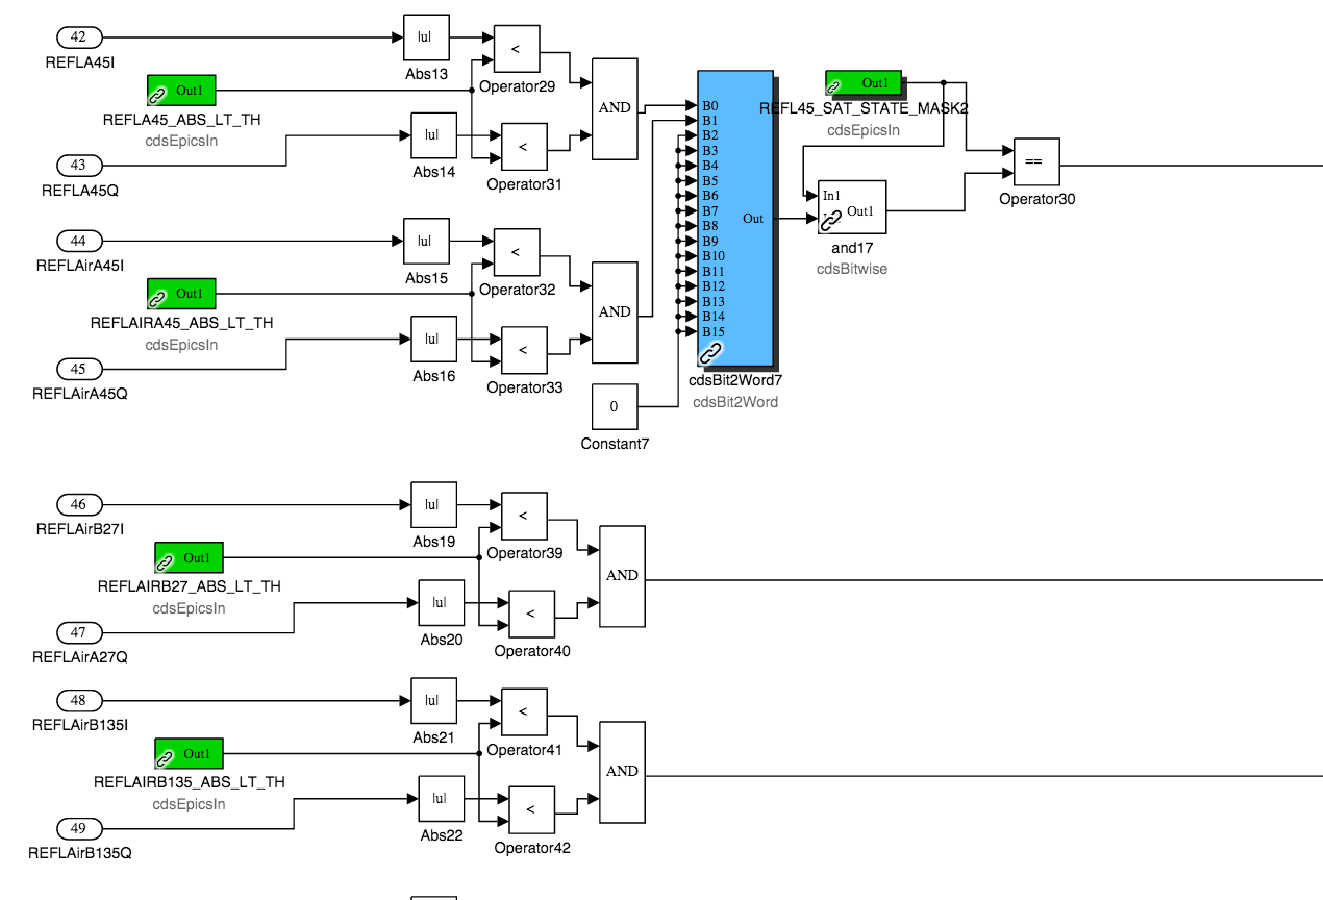
\includegraphics[width=\textwidth]{figures/ODC/LSC-ODC-model}
\caption[LSC ODC SIMULINK Model Example]{Example of LSC ODC bits implemented in SIMULINK}
\end{figure}\label{fig:lsc-odc-model}

\subsection{MEDM screens}

Figure \ref{fig:lsc-odc} shows the LSC ODC overview screen in MEDM.

\begin{figure}[ht!]
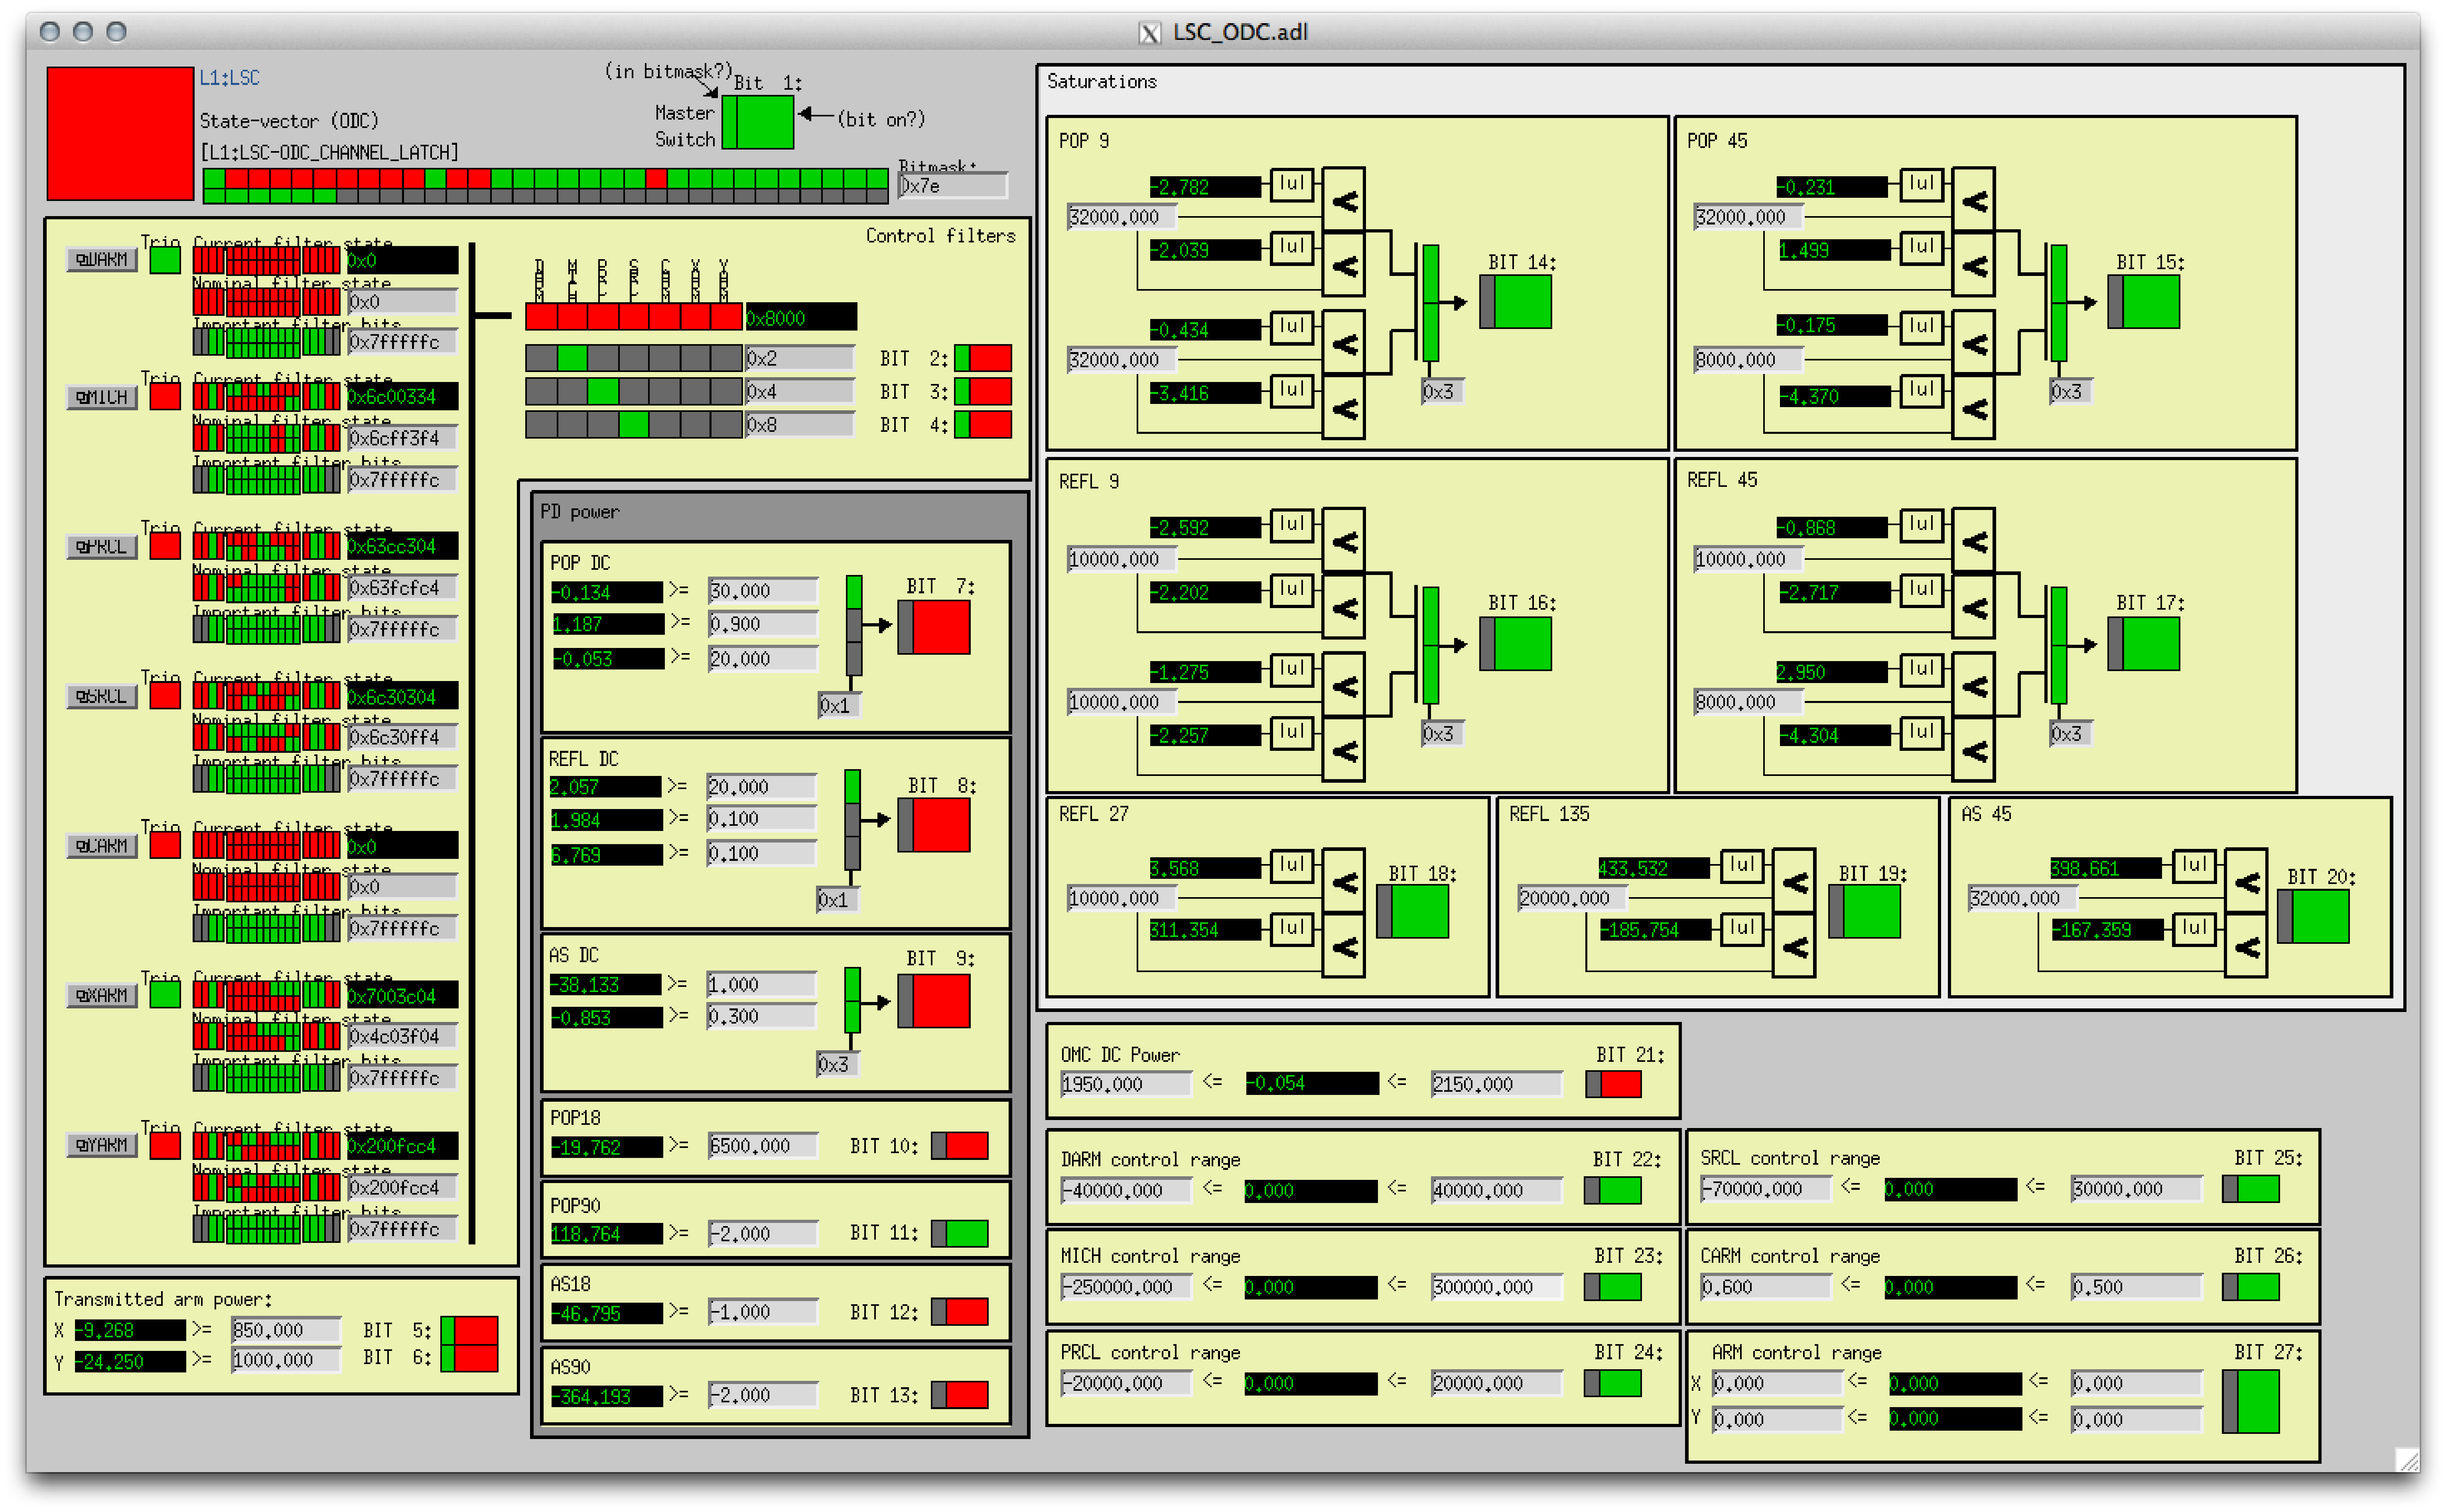
\includegraphics[width=\textwidth]{figures/ODC/LSC_screen}
\caption[LSC ODC Overview Screen]{MEDM screen used to control LSC ODC}
\end{figure}\label{fig:lsc-odc}

\subsection{Summary pages}
I made them

\section{Alignment Sensing and Control}

\subsection{Alignment locking basics and description of threshold signals}

Describe what I did

\subsection{MEDM screens}

Figure \ref{fig:asc-odc} shows the ASC ODC overview screen in MEDM.

\begin{figure}[ht!]
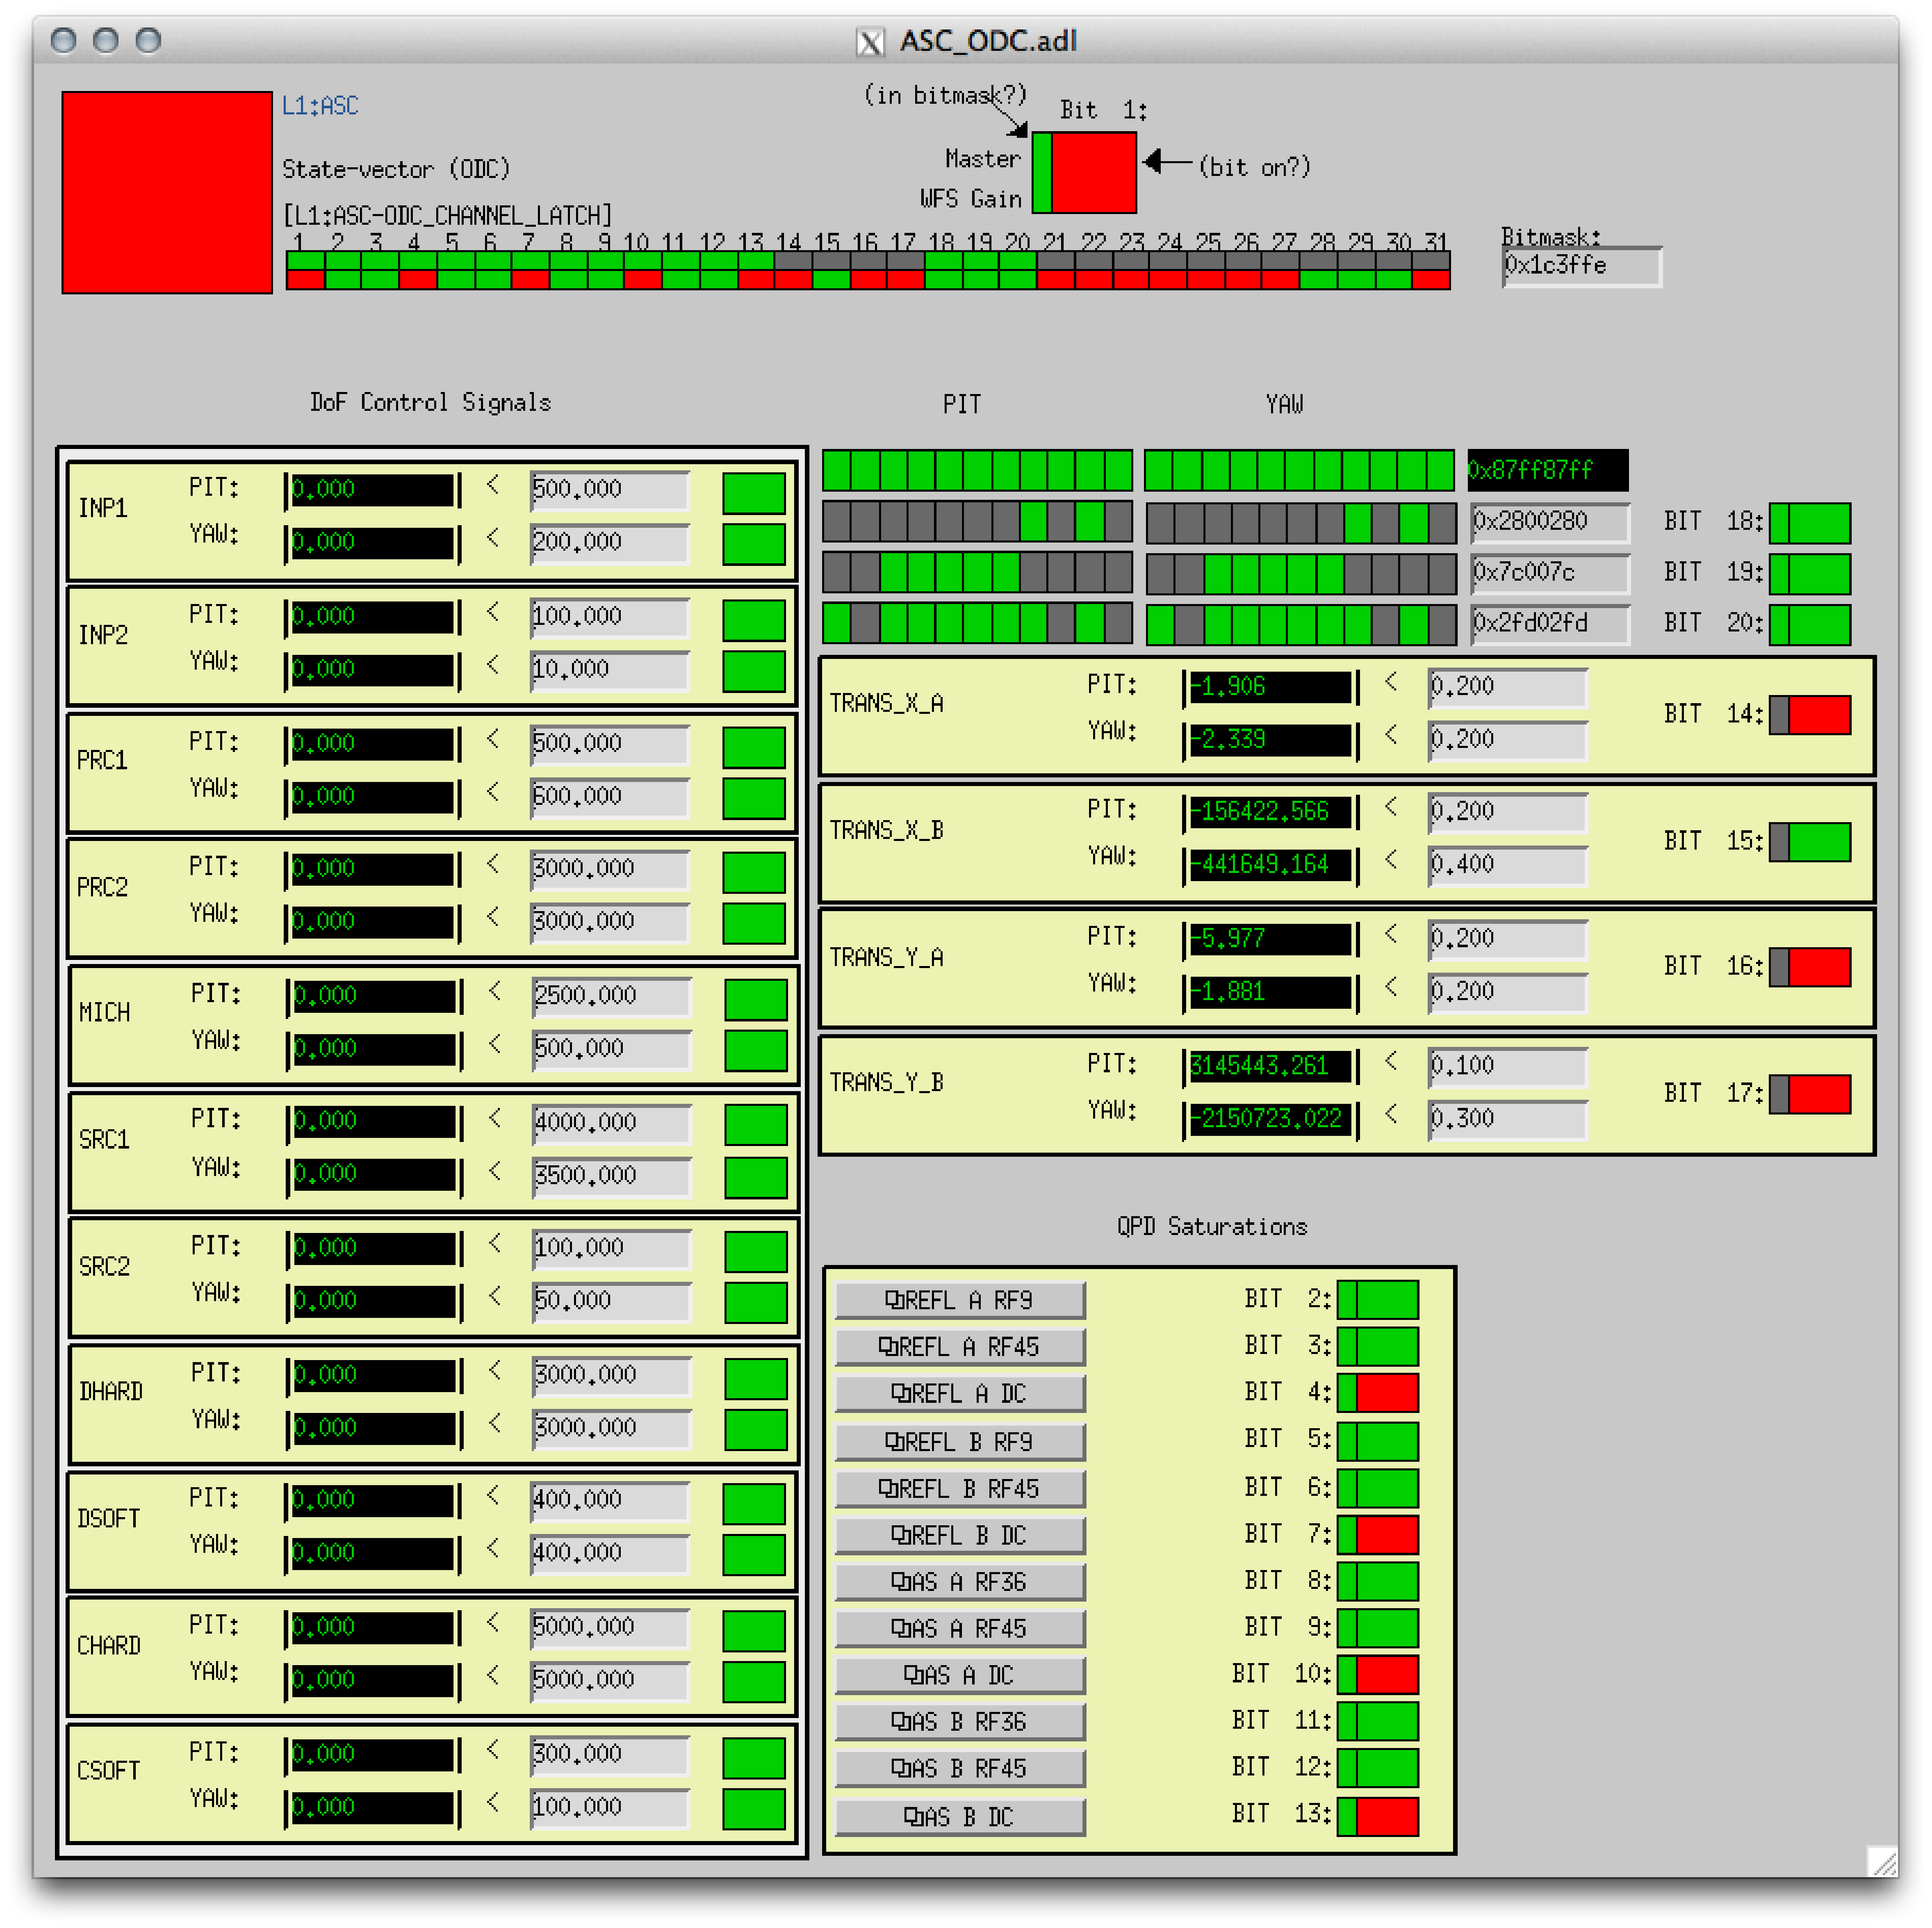
\includegraphics[width=\textwidth]{figures/ODC/ASC_screen}
\caption[ASC ODC Overview Screen]{MEDM screen used to control ASC ODC}
\end{figure}\label{fig:asc-odc}

Figure \ref{fig:odc-pd-screen} shows a photodiode monitor screen in the ASC ODC. 

\begin{figure}[ht!]
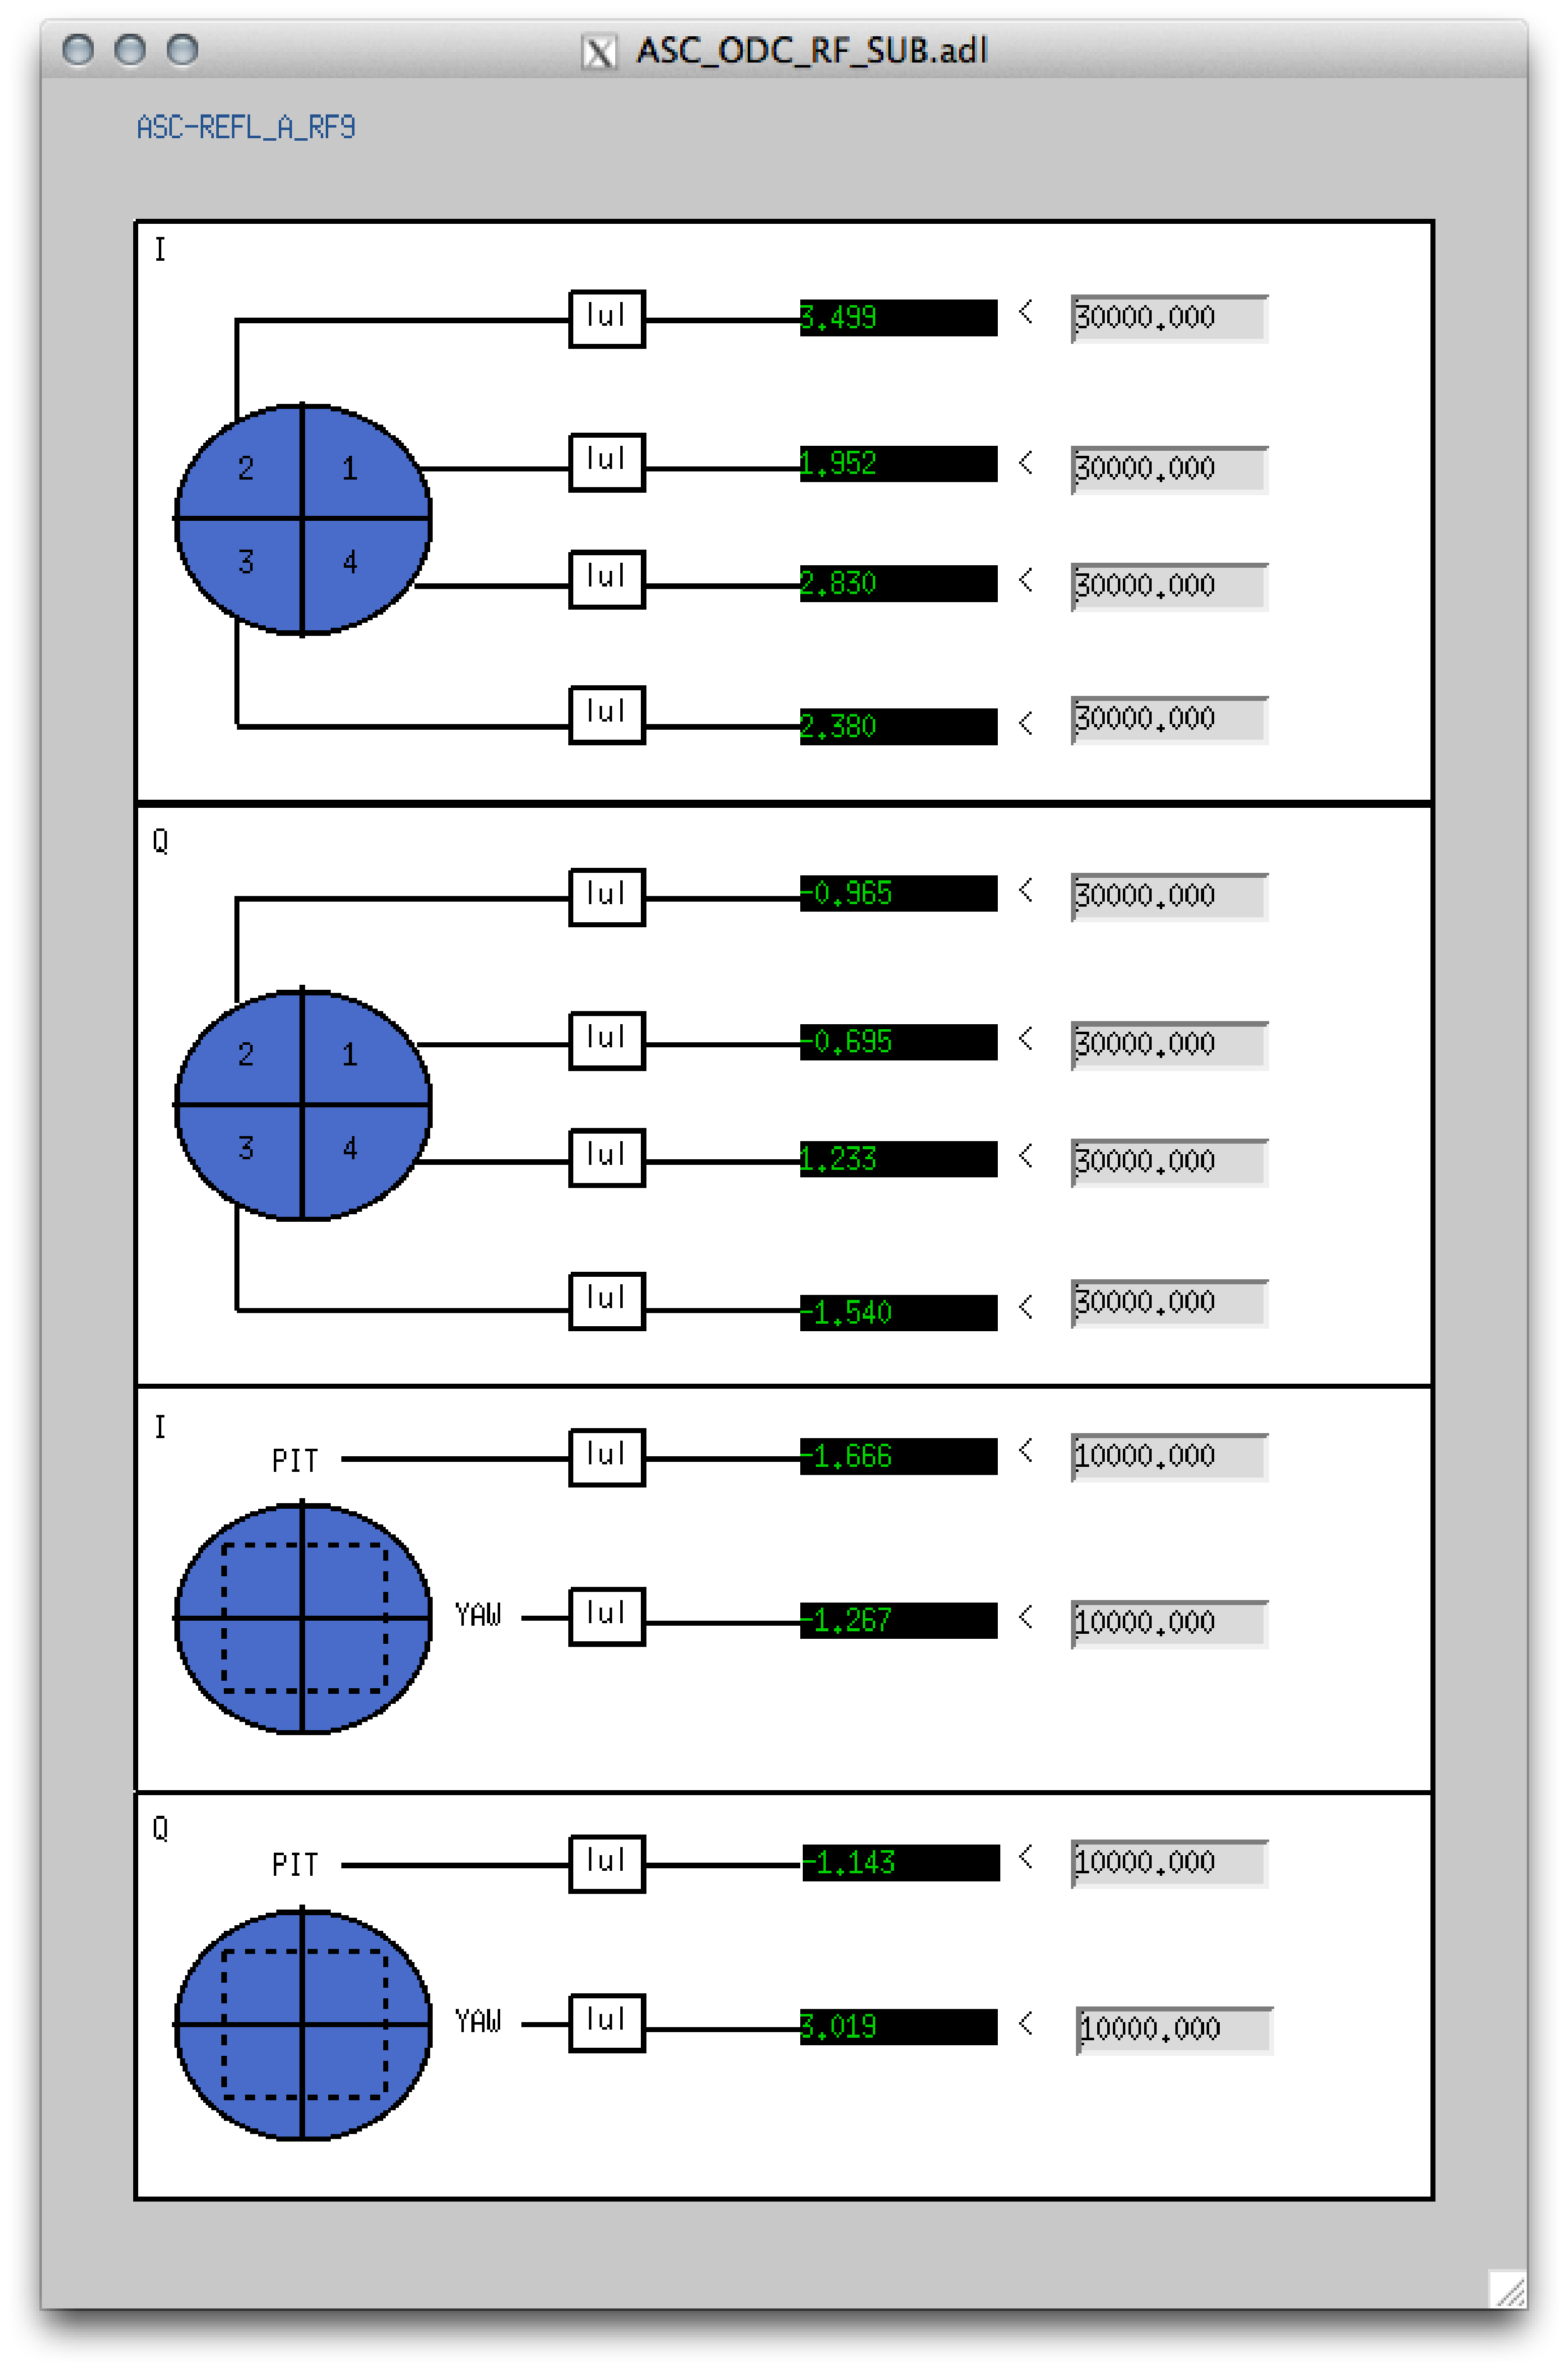
\includegraphics[width=\textwidth]{figures/ODC/PD_screen}
\caption[ASC ODC Photodiode Monitor in MEDM]{ODC monitor for ASC photodiode in MEDM}
\end{figure}\label{fig:odc-pd-screen}

\subsection{Summary pages}
I made them

\section{Results}

We've been able to use ODC for a few interesting things.

\subsection{MICH ODC as a witness of RF45 glitches}

RF45 glitches cause MICH to wiggle, can flag on this for a veto. 

Include VET results for MICH on Omicron triggers.

\subsection{Using alignment flags as a pre-lockloss flag}

Tuned thresholds seem to be decent lockloss predictors.

Measure difference between segment end times and locklosses, histogram values


